\section{Literature Review}

\subsection{Software Traceability and Automated Link Recovery}
Software traceability, the process of establishing and maintaining connections between related software artifacts, is fundamental to understanding, evolving, and maintaining complex software systems~[1],~[2]. It enables effective impact analysis~[3], assists in bug fixing and project management~[5], and is critical to ensuring safety in mission-critical domains~[4].  
A particularly important dimension of traceability is \textbf{issue–commit linking}, which connects issues reported in tracking systems (such as Bugzilla~[9]) to the commits in version control systems (such as Git~[11]) that address them~[6]–[8].\\

While developers can manually reference issue identifiers within commit messages, this practice is inconsistent, leading to missing or incomplete links~[13]. Such gaps obscure the rationale behind code changes and increase maintenance costs~[14]–[16]. Consequently, establishing reliable automated links is vital for downstream research areas such as bug prediction~[17] and commit analysis~[18].  
Over the past two decades, automated approaches to issue–commit linking have evolved from early rule-based systems~[17],~[19],~[20], to classical machine-learning models~[21]–[25], and more recently to deep learning and transformer-based frameworks~[7],~[26]–[31] that capture deep semantic relationships between textual and code artifacts.

\subsection{Rule-Based and Heuristic Approaches}
Early attempts at automated link recovery relied on explicit rules and heuristics, mainly exploiting textual similarity between issue descriptions and commit messages.
\begin{itemize}
    \item \textbf{LINKSTER: Query-Based Manual Inspection} --- Bird \textit{et al.}~\cite{linkster} highlighted the tedious manual effort required to identify missing links and introduced \textbf{LINKSTER}, a tool that facilitated this process by providing query interfaces over issue and commit data. Although LINKSTER simplified retrieval, it relied heavily on manual inspection and lacked full automation.
    \item \textbf{ReLink: Early Automation using Textual Similarity} --- Wu \textit{et al.}~\cite{relink} developed \textbf{ReLink}, considered the first automated approach for recovering missing links through textual similarity. Treating issue reports and commit messages as plain text enabled feature extraction via token frequency and cosine similarity. However, its exclusive reliance on lexical overlap limited its ability to detect semantically related but lexically dissimilar pairs.
    \item \textbf{MLINK: Incorporating Structural (Source-Code) Information} --- Nguyen \textit{et al.}~\cite{mlink} introduced \textbf{MLINK}, extending ReLink by combining textual features with structural information from modified source code. By analyzing actual code changes, MLINK integrated linguistic and syntactic cues, significantly improving precision over purely text-based approaches.
    \item \textbf{RCLinker: Leveraging Generated Commit Messages} --- \textbf{RCLinker}~\cite{q3} addressed the problem of missing or poor-quality commit messages by incorporating automatically generated commit summaries from ChangeScribe~\cite{r27,r28}. By fusing generated and developer-written messages, RCLinker used a random-forest classifier to estimate the likelihood of a link, achieving higher accuracy than heuristic systems.
    \item \textbf{FRLink: Incorporating Non-Source Documents} --- \textbf{FRLink}~\cite{r56} broadened the analysis to include non-source artifacts such as documentation and build scripts that accompany commits. Through contextual filtering, FRLink captured additional signals ignored by purely source-centric methods, improving recall without compromising precision.
    \item \textbf{PULink: Positive-Unlabelled (PU) Learning} --- Recognizing that most unlinked pairs are not truly negative but unlabelled, \textbf{PULink}~\cite{q4} reframed the problem as a Positive-Unlabelled task. This perspective allowed better discrimination between true negatives and unlabeled examples, improving generalization and robustness.
    \item \textbf{HybridLinker: Fusing Textual and Non-Textual Classifiers} --- \textbf{HybridLinker}~\cite{q2} combined textual and structural classifiers using an ensemble model. A weighted fusion of predictions from both sources yielded higher precision and reduced computational overhead, illustrating the benefit of hybrid feature spaces in link recovery.
\end{itemize}

\subsection{Deep Learning and Transformer-Based Approaches}
Recent advances leverage deep neural networks and pre-trained transformers to model complex, non-linear semantic relationships between issues and commits.
\begin{itemize}
    \item \textbf{DeepLink: Code Knowledge Graphs} --- \textbf{DeepLink}~\cite{q1,rene3} was one of the first deep models for issue–commit recovery. It proposed a code knowledge-graph representation to preserve semantic information that is often lost in text-only or bag-of-words models, enabling deeper contextual understanding of commits and their associated issues.
    \item \textbf{T-BERT: Transfer Learning for Data Scarcity} --- \textbf{T-BERT}~\cite{rene4} adopted transfer learning to mitigate limited labeled data in software repositories. By fine-tuning BERT on issue–commit datasets, it achieved notable improvements over traditional machine-learning baselines with minimal domain-specific supervision.
    \item \textbf{BTLink: Dual-Encoder Fusion Architecture} --- \textbf{BTLink}~\cite{btlink} advanced transformer-based models through dual BERT encoders for issues and commits, merged via a fusion layer. This architecture enhanced cross-project adaptability and provided better semantic matching.
    \item \textbf{EALink: Knowledge Distillation and Contrastive Learning} --- \textbf{EALink}~\cite{ealink} focused on efficiency and representation quality through knowledge distillation and contrastive learning. It reduced model size while retaining high accuracy, addressing scalability issues in large repositories.
\end{itemize}

\subsection{Research Gap in Existing Link-Recovery Methods}
Despite these advances, most studies continue to model the problem as a \emph{one-to-one binary classification} task. In practice, software issues are often resolved across multiple commits, each addressing partial aspects such as refactoring, testing, or incremental fixes. Existing frameworks—including advanced transformer-based ones—fail to model these \emph{one-to-many relationships}, leading to incomplete traceability.  
Furthermore, current datasets and evaluation protocols assume a single best commit per issue, reinforcing this oversimplification. The absence of inter-commit relationship modeling also limits downstream tasks such as commit clustering, bug root-cause reasoning, and automated fix generation.  
Hence, there exists a critical gap: the need for a scalable, explainable, and automation-ready model that captures \textbf{multi-commit traceability} and \textbf{causal link reasoning}.

\subsection{Explainability in Software Engineering}
Explainability has emerged as a key pillar of modern software-engineering AI systems. Beyond generating predictions, models must justify their reasoning to support developer trust, auditing, and debugging.  
In the context of traceability, explainable models can articulate why a commit is linked to an issue—by citing specific textual or structural evidence—thereby bridging the gap between automated inference and human comprehension.  
Recent explainable approaches incorporate attention visualization, natural-language rationales, and code summarization to elucidate linking decisions. Such transparency is essential for integrating automated systems into collaborative software environments.

\subsection{Agentic AI for Software Automation}
\subsubsection*{Rise of Agentic AI}
Agentic AI marks a shift from static large-language-model (LLM) interfaces to autonomous, goal-driven agents capable of planning, acting, and reasoning over extended tasks. These agents possess memory, environmental awareness, and tool-use capabilities. In software engineering, this paradigm enables systems that can autonomously analyze repositories, generate code patches, perform testing, and iteratively improve solutions.\\

Practical, developer-facing systems also reflect this agentic trend. Tools such as GitHub Copilot, Anthropic's Claude (including Claude Code variants), Cursor, and Windsurf provide varying degrees of workspace-aware assistance — from context-sensitive code completion and intelligent search to higher-level code generation and refactoring suggestions. While not all of these systems are full multi-step autonomous agents, they illustrate how LLM-powered assistants are being embedded into IDEs and developer workflows, lowering the barrier to broader agentic automation in everyday software maintenance.

\subsubsection*{Multi-Agent Frameworks in Software Maintenance}
Multi-agent frameworks coordinate specialized agents to emulate collaborative developer workflows. By dividing responsibilities—such as task decomposition, code generation, review, and validation—these frameworks achieve scalability and robustness. They also naturally support feedback loops that approximate team-based software maintenance processes.

\subsection{MAGIS: Multi-Agent GitHub Issue Resolution}
\textbf{MAGIS}~\cite{magis} exemplifies the integration of LLM-based agents for end-to-end issue resolution. The framework comprises four primary agents:

\begin{itemize}
    \item \textbf{Manager Agent} -- Acts as the planner and coordinator: it decomposes a reported issue into concrete subtasks, prioritizes work, and either assigns those tasks to existing Developer agents or dynamically designs a team of Developer agents tailored to the problem. This adaptive team-construction improves flexibility and ensures the right mix of skills is assembled for diverse issues.
    \item \textbf{Repository Custodian} -- Responsible for efficient context retrieval within large codebases: the custodian locates relevant files, functions, and hunks that pertain to the issue and prepares compact summaries for downstream agents. Because full-repository querying is costly and LLM context windows are limited, the custodian relies on indexing, selective retrieval, and caching to present focused evidence to other agents.
    \item \textbf{Developer Agents} -- Implement and modify code in a structured, parallelizable workflow: developers generate candidate patches, apply targeted edits, and decompose complex modifications into smaller sub-operations (e.g., generate, refactor, adapt). By separating generation from precise edit application, Developer agents leverage automated code synthesis.
    \item \textbf{QA Engineer Agent} -- Provides task-specific validation and feedback through reasoning and automated testing, paired with each Developer agent to ensure timely reviews. This focused QA pairing shortens review latency, improves patch quality, and enforces testing prior to integration.
\end{itemize}

\begin{figure}[h!]
    \centering
    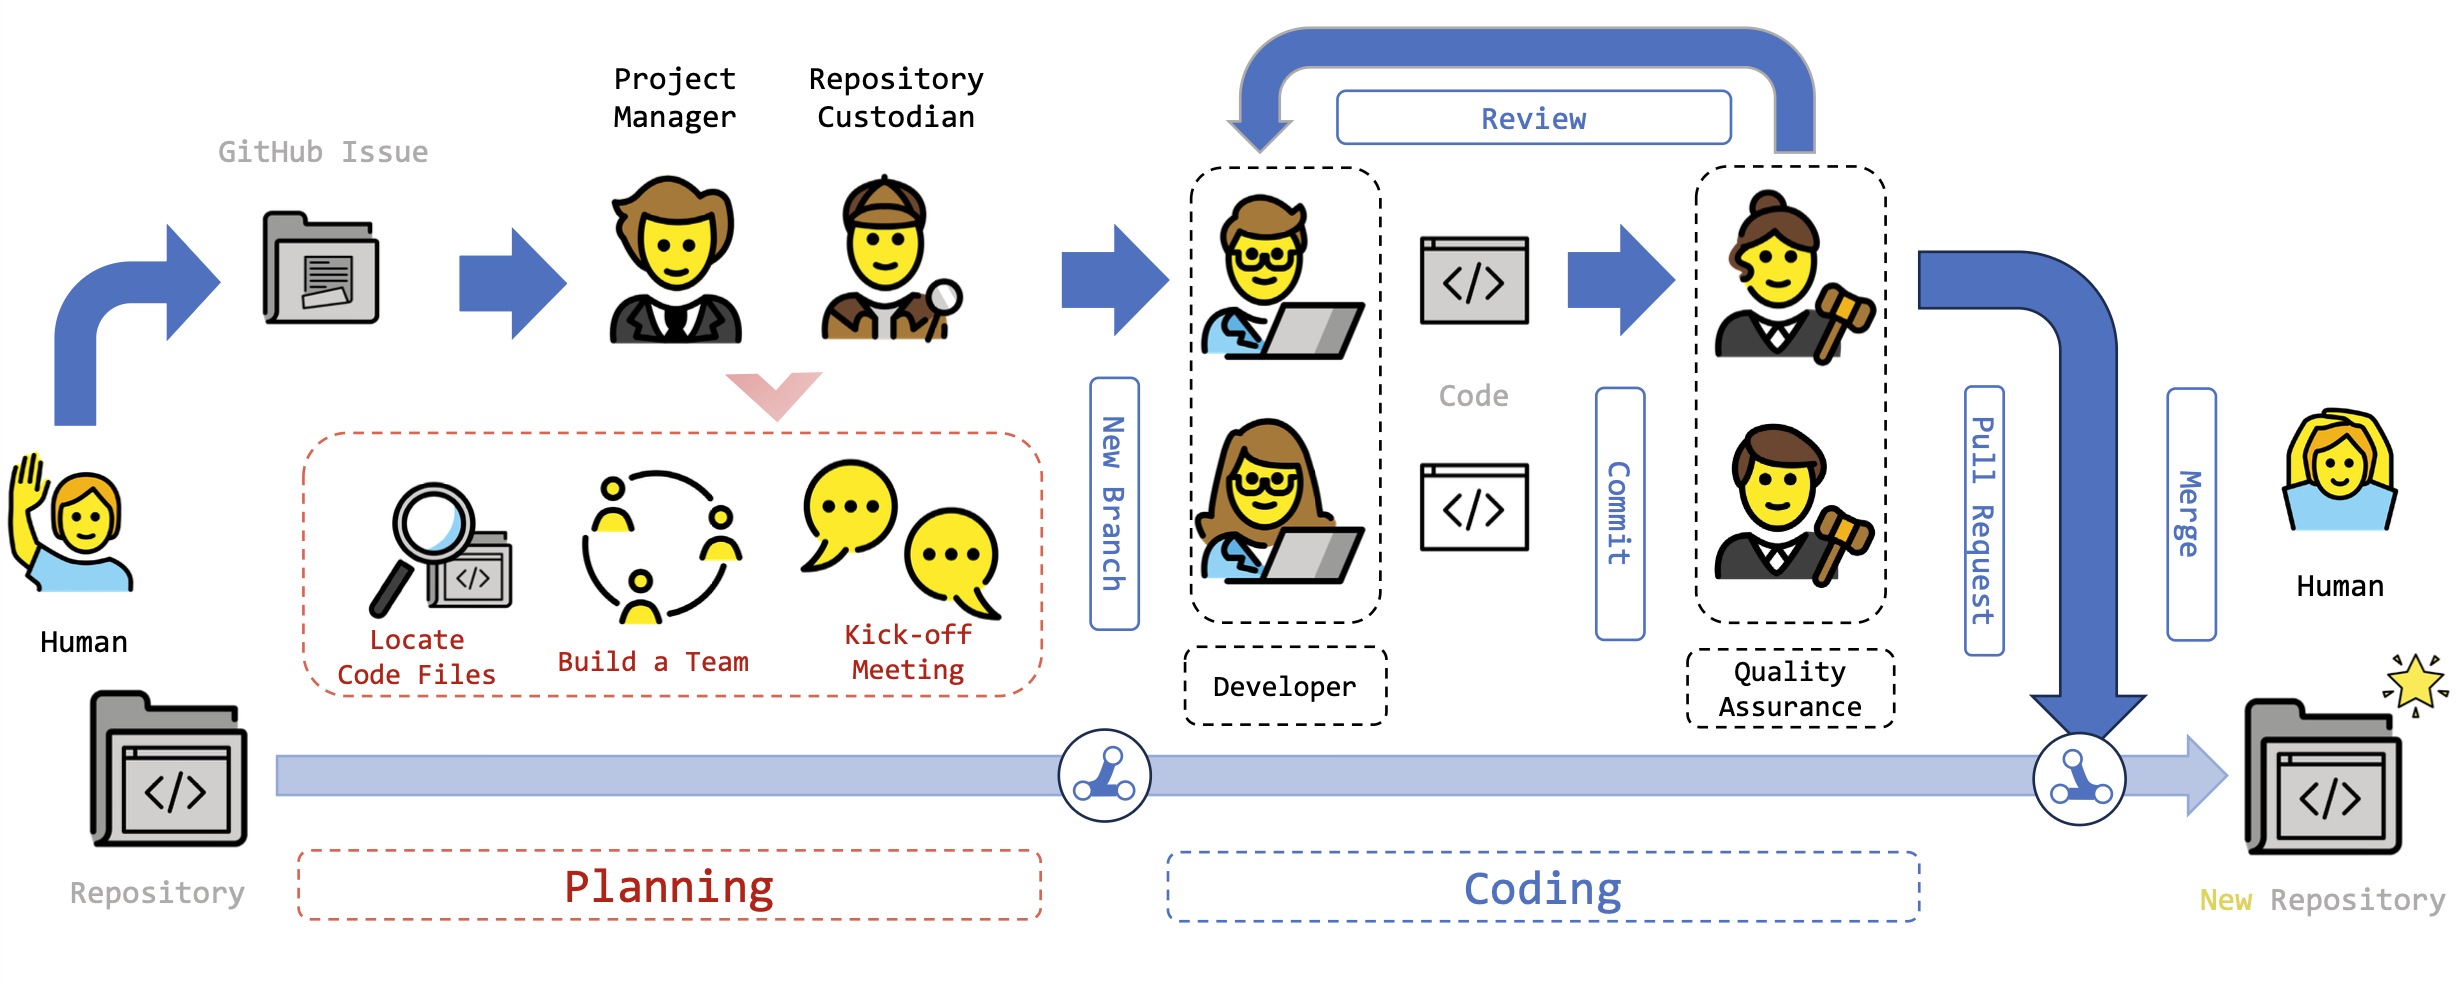
\includegraphics[width=0.88\textwidth]{figures/magis-architecture.png}
    \caption{Architecture of the MAGIS Multi-Agent Framework for GitHub Issue Resolution.}
    \label{fig:magis_architecture}
\end{figure}

MAGIS overcomes three major limitations in prior LLM-based repair systems:
(1) lack of fine-grained localization,  
(2) inability to reason about multi-file dependencies, and  
(3) absence of iterative validation.  
Evaluated on the SWE-Bench benchmark, MAGIS achieved an accuracy of 13.94\%, representing an eight-fold improvement over baseline GPT-4 performance.



\subsection{Proposed Work}
This literature review shows that, despite substantial advances in both traceability and agentic code-repair systems, the two areas remain largely disconnected. Traditional link-recovery approaches provide robust traceability but often lack explainability and automation; agentic systems (e.g., MAGIS) enable automated fixing but typically operate without explicit traceability grounding. Bridging these paradigms calls for a unified framework that combines interpretable trace links with automated repair capabilities.\\Accordingly, we propose a threefold objective for future research in agentic software maintenance:
\begin{enumerate}
    \item robust \textbf{issue--commit traceability} that explicitly models one-to-many relationships between issues and commits using a learning-to-rank approach;
    \item \textbf{explainability mechanisms} that justify link predictions by citing the specific parts of an issue addressed by each commit in natural language; and
    \item \textbf{agentic automation for bug resolution} to propose and, where appropriate, implement fixes guided by traceability evidence and rationales generated by the explainability layer.
\end{enumerate}
\begin{center}
\begingroup
\setlength{\fboxsep}{6pt}% adjust padding as needed
\fbox{%
    \begin{minipage}{\linewidth}
        \textbf{Scope Statement:} This thesis focuses on and covers the major part of Task 1 only — namely, the design, implementation, and evaluation of explainable, multi-commit issue–commit traceability. Broader concerns such as explainability and multi-agent bug fixing frameworks are discussed as future work.
    \end{minipage}%
}
\endgroup
\end{center}
